\documentclass{article}

\usepackage{xeCJK}

% Formatting
\usepackage{geometry}
\usepackage{titling}
\usepackage{parskip}
\usepackage{float}
\usepackage{tocloft}

% Figures
\usepackage{graphicx}
\usepackage{tikz}
\usepackage{pgfplots}
\usepackage{subcaption}

% Math formulas
\usepackage{amsmath}
\usepackage{esint}

% Hyper refs
\usepackage[hidelinks]{hyperref}

% Bibliography
\usepackage[style=authoryear,backend=bibtex]{biblatex}
\usepackage{filecontents}
% Enlarge the outer brackets of nested formulae.
\delimitershortfall=-1pt

% Bibliography.
\bibstyle{eg-alpha-doi}

% Pseudo code.
\lstdefinestyle{pseudo}{
	mathescape=true,
	extendedchars=true,
	frame=tB,
	breaklines=true,
	tabsize=2,
	numbers=left,
	numberstyle=\tiny,
	basicstyle=\scriptsize,
	keywordstyle=\color{black}\bfseries\em,
	keywords={
		input, output,
		function, datatype,
		return, yield, continue, break
		for, foreach, while,
		do, in, done,
		in, on, from, to,
		if, else,
		begin, end,
		new, delete,
		add, apply,
	},
	numbers=left,
	xleftmargin=.04\textwidth,
}
\newenvironment{keywords}{
	\begin{paragraph}{Keywords}
}{
	\end{paragraph}
}

\settoggle{redaction}{true}

\title{A Generic Monte-Carlo Framework for Real-time Simulation of Rigid Body Motion Through Force Fields}
\author{\begin{redacted}Nianyi Wang\end{redacted}}
\date{}

\addbibresource{references.bib}

\begin{document}

\maketitle

\begin{abstract}
	\lorempar[1]
\end{abstract}

\begin{keywords}
	physical simulation;
	Monte-Carlo;
	force field;
	rigid body
\end{keywords}

\section{Introduction}

In real-time applications like video games, it is sometimes necessary to simulate the motion of objects moving through physical fields, such as how a low-density object in water would float due to the buoyancy force.
With regular methods, making frequent queries to the geometrical shape of the simulated object is sometimes inevitable to ensure the realism of the simulation.
Such queries could go on at a frequency of many times per object per frame.
The underlying calculation to perform such simulation would require the geometry information of the target objects, but common game engines don't provide well-encapsulated interfaces for it due to the consideration of runtime performance.
It'd be easy to run into performance issues if one were to implement these queries from scratch.

In this article, we propose a generic framework to compute this type of simulation in a unified way based on the Monte-Carlo method.
It exposes a set of well-encapsulated interfaces for downstream developers to customize for the desired kind of physical field;
it is also possible to tweak the parameters to balance between simulation quality and performance.

The idea of this article originates from simulating the buoyancy behavior of objects submerged in water, so we will be introducing our method mainly with water simulation as a concrete situation.

\section{Related Works}

Speaking in the field of water simulation, the exisiting methods could be divided into two parties: the Lagrangian method, which models water into individual particles and simulates the physical behavior of each, and the Eulerian method, which treats the entire water body as a continuous region and represents it as a field \cite{GOU09}.
Most of the researches on these methods focus on simulating either water itself or the two-way physical coupling between water and submerged objects;
but in this research, we mainly focus on the one-way effect caused on the objects by the field.
The Lagrangian method would have little contribution to our goal, so we will scope on only the Eulerian method.

\cite{teng2016eulerian} proposed a algorithm entirely based on the Eulerian approach, for simulating the two-way coupling between deformable solids and incompressible fluid.
This algorithm could achieve the goal of recreating the realism well, but is too slow for real-time applications, as it would take seconds for a single frame to be rendered.

\cite{GER13} and \cite{BAJ20} proposed algorithms for real-time simulation, but both are based on proxy-based approximation of different manners.
\cite{GER13} takes the entire fluid volume as the induced field of a
limited amount of "panels"---essentially generating seeds at certain location that represent the surrounding fluid motion in their adjacent spaces.
It is cheap enough to run at a real-time scale in a 2D game, but sacrifices the accuracy from reducing the freedom of the fluid’s behavior.
\cite{BAJ20} disects the submerged objects into inter-connected virtual containers.
When an object is submerged in water, the algorithm would simulate the gradual change of water floating into the containers, thus creating a sinking effect.
This algorithm is also cheap enough to be run in real-time, but requires all objects that would be submerged to be equipped with manually-configured virtual container setup.

There were two Monte-Carlo fluid simulation algorithm (\cite{sugimoto2024velocity} and \cite{rioux2022monte}) proposed in recent years, but they are all fluid solvers, not capable for handling the physical effect on objects moving through.

\section{Method}

Let us start with the following observation:
Rigid bodies are treated as point masses in many cases because the precise shapes don't matter, but in the case of simulating their behavior moving through a medium field, they do matter.
To take an example---when a wooden plank falls into water, one side of it first touches the water, and the buoyancy force causes a torque, causing the plank to pitch (fig. \ref{fig:plank-falling-into-water-illustration}).
Had the plank taken as a simple point mass, the torque couldn't have been reflected;
also, the buoyancy force would have only taken effect after the center of mass of the plank passes the water surface.

\begin{figure}[h]
	\def\ih{1in}
	\centering
	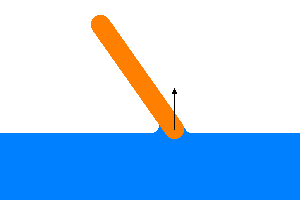
\includegraphics[height=\ih]{../Thesis/figures/stages-of-a-plank-falling-into-water/1.png}
	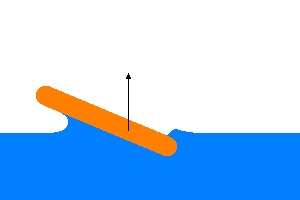
\includegraphics[height=\ih]{../Thesis/figures/stages-of-a-plank-falling-into-water/2.png}
	
\includegraphics[height=\ih]{../Thesis/figures/stages-of-a-plank-falling-into-water/3.png}
	\caption{The stages of a plank falling into water.}
	\label{fig:plank-falling-into-water-illustration}
\end{figure}

To ensure that the result is correct, the entire volume of the rigid body should be taken into consideration.
This sounds computational heavy, but luckily there is the \emph{divergence theorem} to simplify the case:
The integral of the divergence of a vector field ($\mathbf{F}$) over a volume ($V$) is equal to the flux of the field on the boundary of the volume (\ref{formula:divergence-theorem}).

\begin{equation}
	\iiint_{V}(\nabla\cdot\mathbf{F})\mathrm{d}V
	=
	\oiint_{\partial V}\left(\mathbf{F}\cdot\hat{\mathbf{n}}\right)\mathrm{d}\partial V
	.
	\label{formula:divergence-theorem}
\end{equation}

When applied on a fully or partially submerged solid object, this could lead to the famous \emph{Archimedes' principle};
but sadly, the derived principle only tells us how strong the buoyancy force is, but missing the torque information.
To gain the torque information, we need to manually break the integral into discretized elements to make sure every bit of information is included.

Comparing to discretizing and summing over the entire volume, it is obviously easier to just process the surface as directed by the right-hand side of (\ref{formula:divergence-theorem}).
The general steps of our method would be:
\begin{enumerate}
	\item Generate a random set of sample points over the surface of an target object.
	\item Calculate the small contributions of each point.
	\item Sum them up while preserving the torque information.
	\item Apply the summed effect on the target object.
\end{enumerate}
This process would be applied per target object (submerged in water) per frame.

\paragraph*{Step 1: Sample point generation}

This could be done by reading the object's mesh geometry data.
As common game engines all convert meshes into polygon soups of triangles, it is natural to pick a random triangle for each sample, and then pick a random point on it.

However, the chances of each triangle being picked will be the same using this approach, which means that smaller triangles would have the same amount of impact as larger triangles, contradicting the common physical sense.
The solution is to grant each sample point a weight that's proportional to the area of the triangle it's on, and the strength of their contributions will be scaled in step 3.

\paragraph*{Step 2: Local contribution calculation}

This step is pretty straight-forward---just calculate the water pressure based on the position and the normal direction of the point.

\paragraph*{Step 3: Summation}

First, the weights need to be applied on the contributions to make them proportional to the areas they represent, but the summation of these area also need to match with the actual surface area of the object.
The reason that the summed area might mismatch with the actual area is that there is no guarantee that each triangle face would be sampled at least once and only once in each round of sampling.
To fix this, multiply every contribution by an additional factor of $\frac{\text{actual area}}{\text{sum of sample areas}}$.

Then, to sum up the contributions, the point they take effect at must be taken into consideration for perserving the torque information.
By basic Newtonian physics, a force applied on a point on a rigid body could be transformed into an equivalent force applied on its center of mass plus a torque.
Formula (\ref{eq:force-transformation}) shows this transformation, in which $\mathbf r$ represents the delta position from the center of mass to the effect point.
\begin{equation}
	(\mathbf f,\mathbf r)_{\text{force on a point}}\mapsto(\mathbf f,\mathbf r\times\mathbf f)_{\text{force-torque tuple}}.
	\label{eq:force-transformation}
\end{equation}

Lastly, to add two force-torque pais together, simply perform vector addition member-wisely.

\paragraph*{Step 4: Applying}

The result from last step would be a single force-torque pair to be applied on the object.
Every mature game engine should provide physical interfaces of applying force and torque on the center of mass of rigid bodys.

\section{Extension and Applications}

The application of this method is not bound to buoyancy---it could be applied on any scenario where a rigid body moves through a field, as long as the effect caused by the field on mass points obeys the divergence theorem---that is, the field should have first-order continuous partial derivatives.

Even if it doesn't have such property, our based method could downgrade to be sampling inside the volume, and the unifying step before/after combining the contributions needs to be correspondingly using the actual volume as the denominator in the scaling factor.

\section{Analysis}

Jitter.

\section{Future Work}

GPU acceleration.

\section{Conclusion}

\section*{Acknowledgement}
\begin{redacted}
This is the first time I have ever written a serious academical article.
It is guaranteed that there will be naive mistakes all over the place.
Please excuse me, thou reader.
If thou hast spotted any mistake, please feel free to contact me at \url{wangnianyi2001@outlook.com}.
My apologies in advance!

Thanks to the team of my graduation project, \emph{Nani Core} (\url{https://github.com/nani-core}).
The idea of this article rose when I was making the water system in the project.
They established the possibilty for this article to happen.
Special thanks to 陈恩晖 (Omnisch) and 张嘉玥 (Limko).
They are two really, really reliable co-workers and good friends of mine.
They have given me the greatest mental and physical support on the project, and an unforgetful memory in my graduation year.

A sample project of the simulation experiment is published at \url{https://github.com/WangNianyi2001/Water-Simulation-2024}.
\end{redacted}

\printbibliography

\end{document}